%%%%%%%%%%%%%%%%%%%%%%%%%%%%%%%%%%%%%%%%%%%%%%%%%%%%%%%
%                File: OLpagelength.tex               %
%                    VERSION: 1.1                     %
%               Date: May 15, 2004 [sdinee]           %
%                                                     %
%    For assistance, contact Joseph Richardson,       %
%    jricha@osa.org                                   %
%                                                     %
%          LaTeX template and instructions for        %
%          length check and submission of OSA         %
%              Optics Letters manuscripts             %
%                                                     %
%                                                     %
% \documentclass[10pt,letterpaper,twocolumn]{article} %
% \usepackage{OL}                                     %
%                                                     %
% (c) 2004 Optical Society of America                 %
%%%%%%%%%%%%%%%%%%%%%%%%%%%%%%%%%%%%%%%%%%%%%%%%%%%%%%%

\documentclass[10pt,letterpaper,twocolumn]{article} %% two column, final layout

%\documentclass[12pt]{article} % single column, double spaced
%\usepackage[tablesfirst,notablist,nomarkers]{endfloat} %% float figs. to back

\usepackage{ol}
\usepackage{hyperref}
\usepackage{amsmath}

\begin{document}

\twocolumn[ %% activate for two-column option

\title{\textit{Optics Letters} template for submission \\ and length-check estimation}

\author{Chris Videll}

\address{Optics Letters Editorial Office, Optical Society of America, \\ 2010 Massachusetts Avenue, NW, Washington, D.C., 20036}

\author{Joseph Richardson}

\address{Optics Letters Manuscript Office, Optical Society of America, \\  2010 Massachusetts Avenue, NW, Washington, D.C., 20036}

% Do not use \email or \homepage here. E-mail and URL can be given just before references.

\begin{abstract}This template, along with associated style files, can be used to approximate typeset \textit{Optics Letters} (OL) pages for purposes of length check. With a few command changes, the two-column version can be disassembled into a single-column double-spaced version suitable for production and submission to OSA. Examples are given of how to account for some of the factors that affect the accuracy of the length estimate: figures, tables, equations, and author affiliations.\end{abstract} 

\ocis{000.0000, 999.9999.}

 ] %% activate for two-column option

\noindent We recommend that authors prepare OL manuscripts to accommodate the \texttt{[twocolumn]} (length-check) option. This will assist both the author and OSA staff in estimating final page count. Preparing the length-check option involves setting tables and figures within the body of the manuscript with appropriate sizing commands and placing the  \verb+\twocolumn[...]+ command around the title\-page elements (as explained \hyperlink{frontmatter}{below}). There are also instructions at the end of the template for setting up author affiliations properly. Once a manuscript has been prepared to resemble final pages, it can easily be reprocessed to change layout for production, float the figures to the back, and generate a list of figure captions. 

\bigskip

Sample code for the preamble is as follows:

\subsection*{LaTeX for length check}
\small
\begin{verbatim}
\documentclass[10pt,twocolumn]{article}
\usepackage{osajnl}
%% Figures should be placed in body 
%% of manuscript and
%% sized appropriately.
\end{verbatim}
\normalsize

\subsection*{LaTeX for submission}
\small
\begin{verbatim}
\documentclass[12pt]{article}
\usepackage[tablesfirst,notablist,
nomarkers]{endfloat} 
%% use endfloat only to float figures 
%% to end and create 
%% list of captions
\usepackage{osajnl}
\end{verbatim}
\normalsize

The command \verb+\twocolumn[...]+ must be placed around the titlepage elements in the two-column option. Note that proper figure, table, and caption environments should be used (see samples below). 

\textbf{Displayed equations} may be the most problematic for purposes of length check. \emph{Optics Letters} equations are usually set in one column; breaks and alignment should bring out the structure of the math:
%% LaTeX 
%\begin{eqnarray}
%{\dot{E}_{x,y}} &=&\frac{1}{2}\left( 1+j\alpha \right) \left( G_{x,y}-\gamma \right) %E_{x,y}  \label{Eq1} \nonumber \\
%&&+\kappa E_{x,y}\left( t-\tau \right) \exp \left( -j\Omega
%_{x,y}\tau \right) \nonumber \\
%&& + (\beta _{sp}N)^{1/2} \xi _{x,y}. 
%\end{eqnarray}

%% amsmath
\begin{align}
{\dot{E}_{x,y}} &=\frac{1}{2}\left( 1+j\alpha \right) \left( G_{x,y}-\gamma \right) E_{x,y}  \label{Eq1} \nonumber \\
&\quad+\kappa E_{x,y}\left( t-\tau \right) \exp \left( -j\Omega
_{x,y}\tau \right) \nonumber \\
&\quad + (\beta _{sp}N)^{1/2} \xi _{x,y}. 
\end{align}


Use standard LaTeX or AMSTeX environments. For equations that \textit{must} span two columns, it is possible to use a float environment, e.g., \verb+\begin{figure*}...\end{figure*}+. Such an environment will not interfere with figure or table numbering (which is controlled by the caption), but it \textit{will} cause equations to float, often with unwanted consequences.

\textbf{Figures} should  be set to one-column size \mbox{($\sim$8.3 cm)} whenever possible; \textbf{tables} should also be set to one column whenever possible, but tables with more than five columns will probably need to be set to two columns. For two-column layout, figures and tables can be set across both columns with the alternate figure and table environment commands \verb+\begin{figure*}...\end{figure*}+ instead of \verb+\begin{figure}...\end{figure}+. Note that tables are typeset and cannot be reduced in size like art, which may require more space than in the submitted paper.

\subsection*{Sample figure environment:}
\small
\begin{verbatim}
\begin{figure}[htb]
\centerline{\includegraphics[width=8.3cm]{sample.eps}}
 \caption{Sample figure.}
\end{figure}
\end{verbatim}
\normalsize

\textbf{References} callouts are formatted with the \texttt{overcite} package, which produces superscript numerical reference callouts. Online callouts, e.g., see Ref. 1, can be produced with the command \verb+\citeonline{}+.

Before submitting, authors who use BibTeX should first run BibTeX, then paste the contents of the output file \texttt{*.bbl} into the \texttt{*.tex} manuscript file. Our electronic submissions system cannot process BibTeX directly. A new BibTeX style file, \texttt{osajnl.bst}, is included in this distribution.

\paragraph{The following files are included in this distribution:}
\begin{itemize}\itemsep-2pt
\item\texttt{OLpagelength.tex} \ Template and instructions 
\item\texttt{OL.sty} \ Style file 
\item\texttt{osajnl.bst} \ BibTeX style file
\item\texttt{endfloat.cfg} \ Configuration file for the \texttt{endfloat} package
\item\texttt{sample.eps} \ Sample .eps figure.
\end{itemize}

\bigskip

\begin{figure}[htb]
\centerline{\includegraphics[width=8cm]{sample.eps}}
\caption{Sample column-width figure; note that multipart figures should be assembled as a single file.}
\end{figure}


\begin{table}
  \centering
  \caption{Sample Table}\begin{tabular}{ccccc} \\ \hline
    % after \\: \hline or \cline{col1-col2} \cline{col3-col4} ...
    TEST & TEST & TEST & TEST & TEST \\ \hline
    TEST & TEST & TEST & TEST & TEST \\
    TEST & TEST & TEST & TEST & TEST \\
    TEST & TEST & TEST & TEST & TEST \\ \hline
  \end{tabular}
\end{table}

\begin{table*}[htb]
  \centering
  \caption{Sample Table}\begin{tabular}{ccccccccc} \\ \hline
    % after \\: \hline or \cline{col1-col2} \cline{col3-col4} ...
    TEST & TEST & TEST & TEST & TEST & TEST & TEST & TEST & TEST\\ \hline
    TEST & TEST & TEST & TEST & TEST & TEST & TEST & TEST & TEST\\
    TEST & TEST & TEST & TEST & TEST & TEST & TEST & TEST & TEST\\
    TEST & TEST & TEST & TEST & TEST & TEST & TEST & TEST & TEST\\ \hline
  \end{tabular}
\end{table*}


\begin{figure*}[t]
\centerline{\includegraphics[width=10cm]{sample.eps}}
\caption{Two-column figure set with the figure* environment.}
\end{figure*}


Dummy text. Dummy text. Dummy text. Dummy text. Dummy text. Dummy text. Dummy text. Dummy text. Dummy text. Dummy text. Dummy text. Dummy text. Dummy text. Dummy text. Dummy text. Dummy text. Dummy text. Dummy text. Dummy text. Dummy text. Dummy text. Dummy text. Dummy text. Dummy text.

Dummy text. Dummy text. Dummy text. Dummy text. Dummy text. Dummy text. Dummy text. Dummy text. Dummy text. Dummy text. Dummy text. Dummy text. Dummy text. Dummy text. Dummy text. Dummy text. Dummy text. Dummy text. Dummy text. Dummy text. Dummy text. Dummy text. Dummy text. Dummy text. 

Dummy text. Dummy text. Dummy text. Dummy text. Dummy text. Dummy text. Dummy text. Dummy text. Dummy text. Dummy text. Dummy text. Dummy text. Dummy text. Dummy text. Dummy text. Dummy text. Dummy text. Dummy text. Dummy text. Dummy text. Dummy text. Dummy text. Dummy text. Dummy text. 

Dummy text. Dummy text. Dummy text. Dummy text. Dummy text. Dummy text. Dummy text. Dummy text. Dummy text. Dummy text. Dummy text. Dummy text. Dummy text. Dummy text. Dummy text. Dummy text. Dummy text. Dummy text. Dummy text. Dummy text. Dummy text. Dummy text. Dummy text. Dummy text. 

Dummy text. Dummy text. Dummy text. Dummy text. Dummy text. Dummy text. Dummy text. Dummy text. Dummy text. Dummy text. Dummy text. Dummy text. Dummy text. Dummy text. Dummy text. Dummy text. Dummy text. Dummy text. Dummy text. Dummy text. Dummy text. Dummy text. Dummy text. Dummy text. 

Dummy text. Dummy text. Dummy text. Dummy text. Dummy text. Dummy text. Dummy text. Dummy text. Dummy text. Dummy text. Dummy text. Dummy text. Dummy text. Dummy text. Dummy text. Dummy text. Dummy text. Dummy text. Dummy text. Dummy text. Dummy text. Dummy text. Dummy text. Dummy text. 

Dummy text. Dummy text. Dummy text. Dummy text. Dummy text. Dummy text. Dummy text. Dummy text. Dummy text. Dummy text. Dummy text. Dummy text. Dummy text. Dummy text. Dummy text. Dummy text. Dummy text. Dummy text. Dummy text. Dummy text. Dummy text. Dummy text. Dummy text. Dummy text. 

Dummy text. Dummy text. Dummy text. Dummy text. Dummy text. Dummy text. Dummy text. Dummy text. Dummy text. Dummy text. Dummy text. Dummy text. Dummy text. Dummy text. Dummy text. Dummy text. Dummy text. Dummy text. Dummy text. Dummy text. Dummy text. Dummy text. Dummy text. Dummy text. 



Dummy text. Dummy text. Dummy text. Dummy text. Dummy text. Dummy text. Dummy text. Dummy text. Dummy text. Dummy text. Dummy text. Dummy text. Dummy text. Dummy text. Dummy text. Dummy text. Dummy text. Dummy text. Dummy text. Dummy text. Dummy text. Dummy text. Dummy text. Dummy text. 


Dummy text. Dummy text. Dummy text. Dummy text. Dummy text. Dummy text. Dummy text. Dummy text. Dummy text. Dummy text. Dummy text. Dummy text. Dummy text. Dummy text. Dummy text. Dummy text. Dummy text. Dummy text. Dummy text. Dummy text. Dummy text. Dummy text. Dummy text. Dummy text. 


Dummy text. Dummy text. Dummy text. Dummy text. Dummy text. Dummy text. Dummy text. Dummy text. Dummy text. Dummy text. Dummy text. Dummy text. Dummy text. Dummy text. Dummy text. Dummy text. Dummy text. Dummy text. Dummy text. Dummy text. Dummy text. Dummy text. Dummy text. Dummy text. 

Dummy text. Dummy text. Dummy text. Dummy text. Dummy text. Dummy text. Dummy text. Dummy text. Dummy text. Dummy text. Dummy text. Dummy text. Dummy text. Dummy text. Dummy text. Dummy text. Dummy text. Dummy text. Dummy text. Dummy text. Dummy text. Dummy text. Dummy text. Dummy text. [use \verb+\pagebreak+ to balance final column]

%\pagebreak
\begin{thebibliography}{99}
\bibitem{Galvan1992} A. Galvanauskas, J.A. Tellefsen Jr., A. Krotkus, M. Oberg, B. Broberg,  Appl. Phys. Lett. {\bf 60,} 145 (1992).

\bibitem{Zhang} Z. Jiang and X.-C. Zhang,  Opt. Lett. {\bf 23,} 1114 (1998).

\end{thebibliography}
\clearpage
\twocolumn[

\hypertarget{frontmatter}{Avoid} using footnotes in affiliations. Authors' names and affiliations should be listed on separate lines instead. 

\vskip5ex

\noindent\textbf{This is not OL style:} 

\author{M. Scott Dineen,$^1$ Joseph Richardson,$^2$ and Chris Videll$^1$. . . }
\affiliation{$^1$ University of Maryland}
\vskip-8pt
\affiliation{$^2$ University of Virginia}

\noindent \textbf{This is OL style:}

\author{M. Scott Dineen}

\address{University of Maryland}

\author{Joseph Richardson}

\address{University of Virginia}

\author{Chris Videll}

\address{University of Maryland}

\bigskip

Rather than using footnotes, list authors affiliated with different departments of the same school or organization should be on separate lines:

\author{M. Scott Dineen}

\address{Department of Physics, University of Maryland}

\author{Chris Videll}

\address{Department of Electrical Engineering, University of Maryland}

\bigskip

Footnotes are acceptable for present addresses

\author{M. Scott Dineen$*$}


\affiliation{University of Maryland}

at the end of the acknowledgment


\centerline{*Present address, University of Virginia}

\bigskip

If URLs are used, they should be added after the author(s) e-mail address(es) in the acknowledgment.
]

\end{document} 